%!TEX root = batch-course.tex

%-------------------------------------------------
\section{Case study: DuPont process}
%-------------------------------------------------

\begin{frame}\frametitle{DuPont Nylon example: learning from new data}

	\begin{itemize}
		\item	Industrial data set of \( N = 55 \) batches from Nylon production
		
		\item	Temperature, pressure and flow rate variables: \( K = 10\)  batch tags
		
		\item	Batch duration about 2 hours (\( J=100 \) time intervals)
		
		\item	12 hours before lab values returned: batch-to-batch adjustment not possible
		
		\item	Known problems with batches: 38, 40, 41, 42, 50, 51, 53, 54, 55
	\end{itemize}
	
	
\end{frame}

\begin{frame}\frametitle{DuPont Nylon example: raw data}
	{\color{myGreen}{Note}}: data were scaled for confidentiality
	\begin{center}
		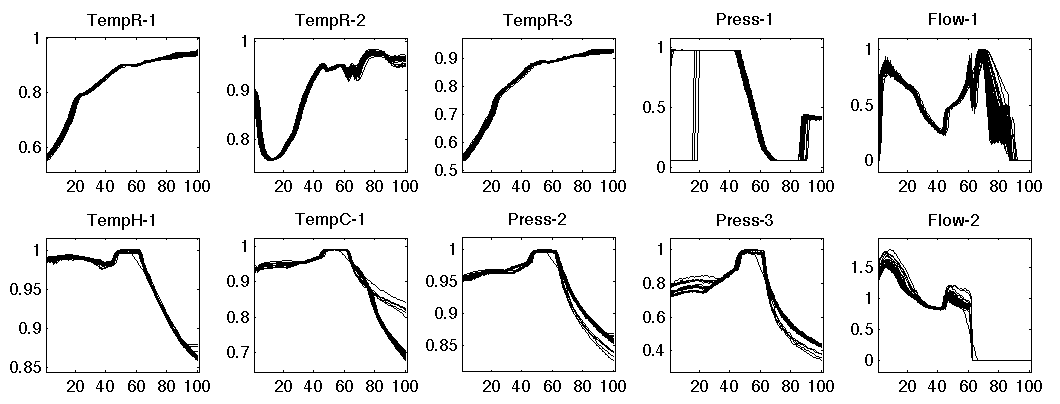
\includegraphics[width=\textwidth]{images/dupont/dupont-raw-data-trajectories.png}
	\end{center}
	
	\vspace{1cm}
	\begin{itemize}
		\item	Can see a few unusual batches: see ``Temp-C1'' and ``Press-1'' tags
		
		\item	Alignment looks pretty good (process is well controlled)
		
		\item	Some periods are noisy: ``Flow-1'' and ``Flow-2''
	\end{itemize}
\end{frame}

\begin{frame}\frametitle{DuPont Nylon example: initial PCA}
	\begin{itemize}

		\item	Just start with 2 components initially
		
				\begin{itemize}					
					\item	no cross-validation, just get a ``feel'' for the data
					\item	\( R^2_X = [38.28\%, 17.58\%]\), or cumulatively: 55.9\%
				\end{itemize}
		
		\item	Score plot: {\color{myOrange}{\texttt{plot(batch\_PCA, 'scores')  }}}
				
				\begin{columns}
					\column{0.8\textwidth}
						\begin{center}
							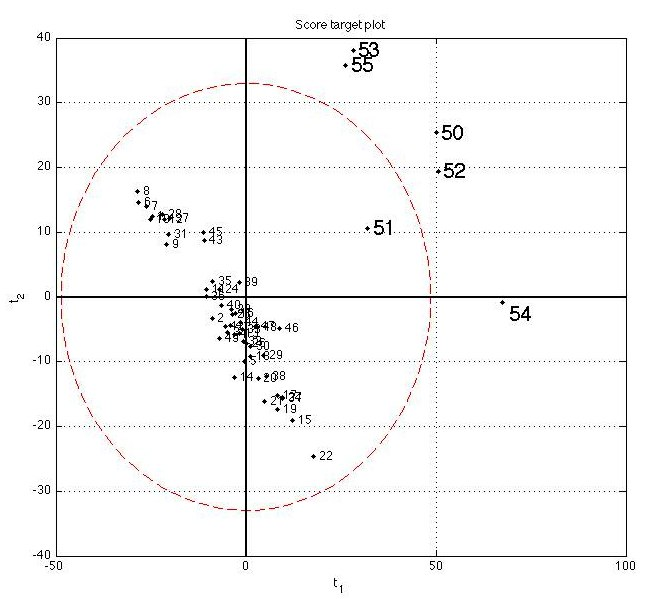
\includegraphics[width=0.8\textwidth]{images/dupont/dupont-raw-score-plot.jpg}
							% batch_PCA = lvm({'X', batch_X}, 2);
							% plot(batch_PCA, 'scores', {'labels'})
						\end{center}
						
					\column{0.4\textwidth}
						\begin{itemize}
							\item	Batches 50 to 55 unusual
							
							\item	Distorted the model		
							
							\item	Before excluding them and rebuilding model, let's first examine them.
						\end{itemize}
				\end{columns}
	\end{itemize}
\end{frame}

\begin{frame}\frametitle{DuPont Nylon example: SPE}
	\begin{itemize}
		\item	SPE plot: {\color{myOrange}{\texttt{plot(batch\_PCA, 'spe')  }}} 
	\end{itemize}
	
	\begin{center}
		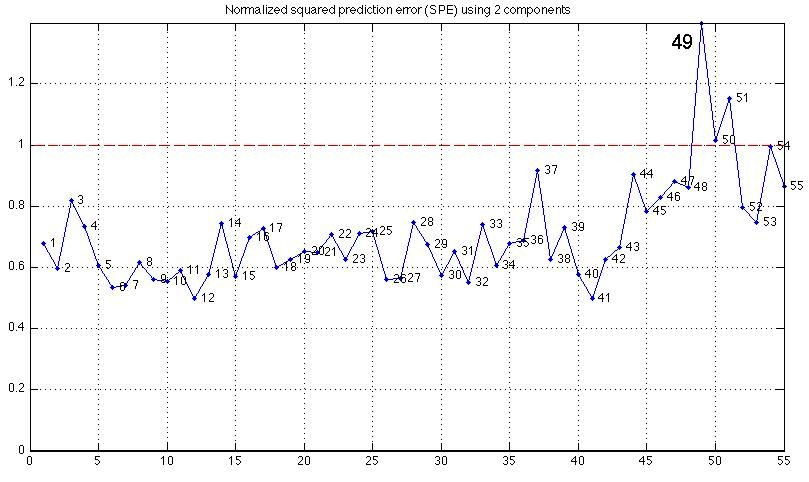
\includegraphics[width=\textwidth]{images/dupont/dupont-raw-SPE.jpg}
	\end{center}
\end{frame}

\begin{frame}\frametitle{DuPont Nylon example: batch 54 (high \( t_1 \) batch)}
	\begin{itemize}
		\item	First plot loadings \( p_1 \) to understand that direction
			
				\begin{itemize}
					\item	{\color{myOrange}{\texttt{plot(batch\_PCA.X, 'loadings', 1)    }}} 
					
					\item	Tags and time periods that are positive in \( p_1 \) will be high in batch 54
					
					\item	The opposite also applies
				\end{itemize}
		
		\item 	Main problems are at the end of the batch:
		
				\begin{itemize}
					\item	Pressures 2 and 3 are below normal
					
					\item	Temp-C1 is above normal
					
				\end{itemize}
		
		\item 	Other problems in Temp-R1 and Temp-R3 at start of the batch
	\end{itemize}
\end{frame}

\begin{frame}\frametitle{DuPont Nylon example: loadings \( p_1 \)}

\begin{center}
	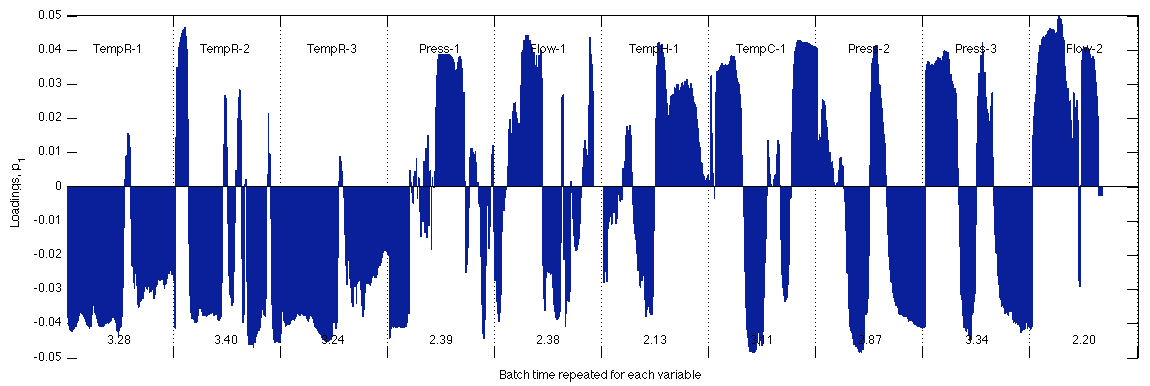
\includegraphics[width=\textwidth]{images/dupont/dupont-loadings-p1.png}
\end{center}

	\begin{itemize}
		\item	Explore other score outliers interactively in class
	\end{itemize}
\end{frame}

\begin{frame}\frametitle{DuPont Nylon example: SPE}

	\begin{itemize}
		\item	Batch 49 shows in the overall SPE 
		
		 		\begin{itemize}
		 			\item	{\color{myOrange}{\texttt{plot(batch\_PCA, 'spe') }}} 
		 		\end{itemize}

		\item 	Also look at the time-varying SPE to see \emph{when} problem occurred: \( t \) = 57 to 67 
		
				\begin{itemize}
					\item	{\color{myOrange}{\texttt{plot(batch\_PCA, 'spe', \{'batch', 49\})  }}} 
				\end{itemize}
		
		\item 	Confirm in contribution plots: tags 6 to 10
	\end{itemize}
	
	\begin{center}
		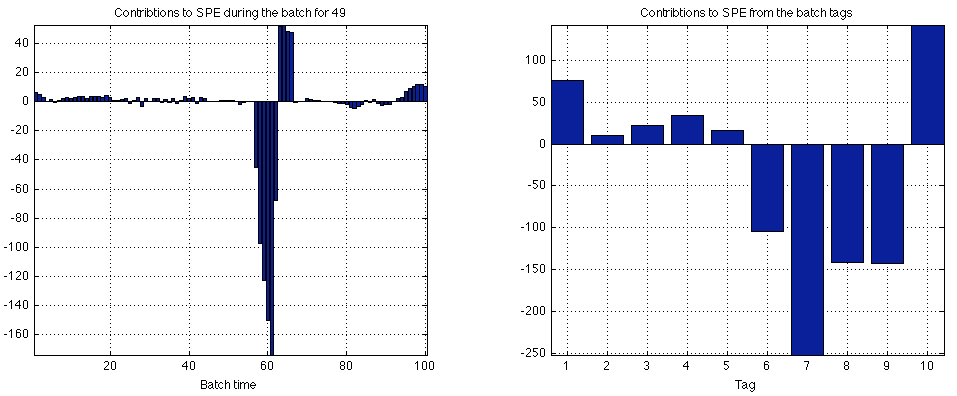
\includegraphics[width=\textwidth]{images/dupont/dupont-batch-49-spe.png}
	\end{center}
\end{frame}

\begin{frame}\frametitle{DuPont Nylon example: Raw data for batch 49}

	\begin{itemize}
		\item	Likely that tag 5 (wrongly) identified as cause
	\end{itemize}
	\begin{center}
		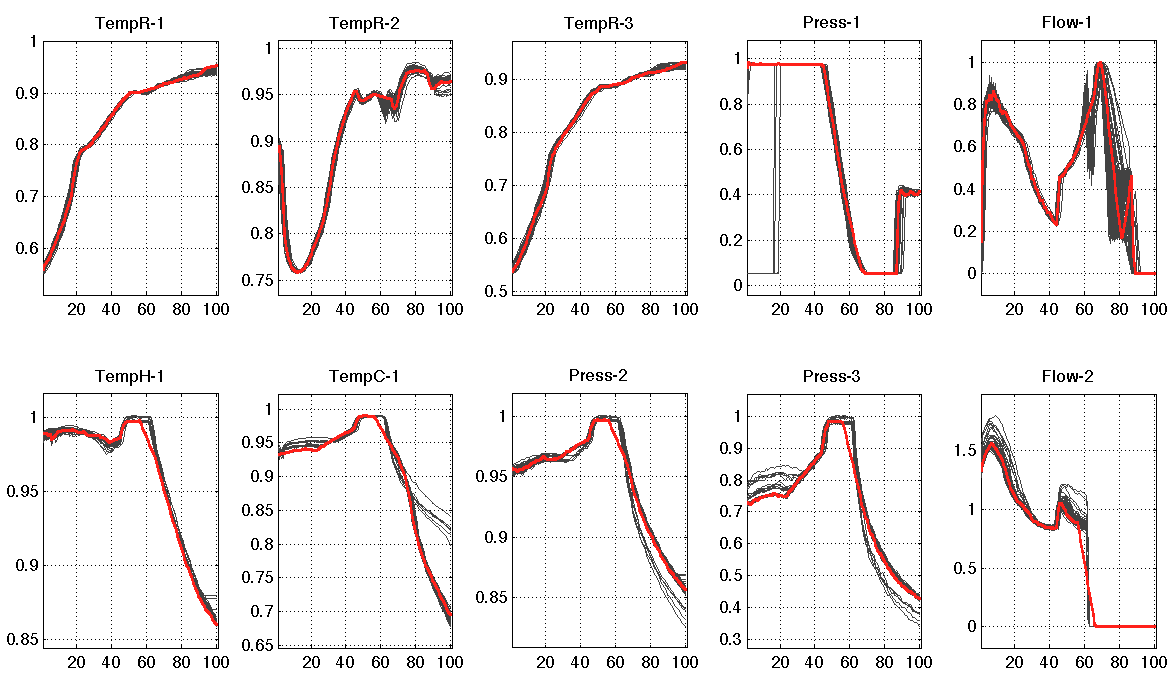
\includegraphics[width=\textwidth]{images/dupont/dupont-highlight-raw-data-batch-49.png}
	\end{center}
	
	\begin{itemize}
		\item	Cause: subtle deviations in heating and cooling system (broken correlation) and pressure system
	\end{itemize}
\end{frame}

\begin{frame}\frametitle{DuPont Nylon example: Exclude and rebuild}

	\begin{itemize}
		\item	Exclude batches 49, 50, ... up to 55 and rebuild
		
		\item	Start to see some other outliers in \( t_2 - t_3 \) 

		\item	We will investigate those interactively in class
	\end{itemize}
	
	
\end{frame}

\begin{frame}\frametitle{DuPont Nylon example: Note}

	\begin{itemize}
		\item	Batches 38, 40, 41 and 42 were known to have problematic final quality (FQAs)
		
		\item	No cause/detection can be found in the plots for these batches
		
		\item	Problems are not present in trajectories
				
				\begin{itemize}
					\item	perhaps not measuring a trajectory
					
					\item	should there be \( \mathbf{Z} \), initial condition data, that we should use?
				\end{itemize}
		
		\item	\textbf{Key point}: online measurements must contain the information required to make a classification (\emph{observability requirement})			
		
	\end{itemize}
	
	
\end{frame}

